\documentclass[a4paper,11pt,titlepage]{jarticle}
\usepackage[dvipdfmx]{graphicx}
\usepackage{listings}
\usepackage{amsmath}
\usepackage{fancybox,ascmac}
\usepackage{url}
\usepackage{here}



\title{知能情報実験I : 第九回レポート}
\author{175751C 宮城孝明}
\date{平成30年6月12日}

\begin{document}
\maketitle
\tableofcontents
\clearpage
\section{実験目的}
 本実験では,簡単な順序回路の設計および実験を行うことによって,
フリップフロップ(FF)の特性を理解するとともに,
カウンタの動作原理および簡単な順序回路の設計方について習得する。
\section{実験概要}
 今回の実験では,FF(フリップフロップ)の特性を理解するために,
実際に順序回路であるフリップフロップの応用であるカウンタの作成を行った。
はじめに,講師から説明を受け事前に順路回路とフリップフロップの知識をつけて
から作業を始めた。簡単な回路設計ではあるが,4進カウンタ回路や3進カウンタ回路
を作成し動作確認を行うことで基本的な仕組みを理解できる。さらに,今回作成する
回路である順序回路は,記憶機能が存在する。そのため,動作を確認する際には,
時間の概念も存在する。そのため,タイミングチャートを用いられた。
そして,オシロスコープも用いて,データの出力とクロック信号を波形上にすることで,
視覚的にわかりやすくなる。

\section{実験結果}
\begin{enumerate}
  \item 実験(1) \par
    D-FF回路は,データの出力である$\overline{Q}$とデータ入力Dを直結すれば,データの入力値は
  その値を回路上でずっと回ることになる。これにより,入力値を覚える回路ができる。今回は,D-FF回路を
  1つだけしか使用してないためともう一つのデータ出力Qが1つのため,この回路は2進カウンタ(1ビットカウンタ)
  と呼ばれる。\par
  \begin{figure}[H]
\centering
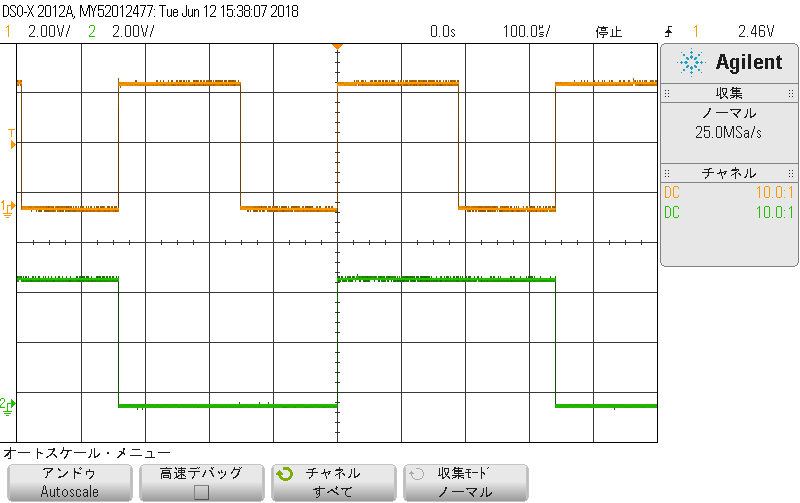
\includegraphics[width=90mm]{scope_2.png}
\label{sample1}\\
\caption{2進カウンタ(1ビットカウンタ)データ出力Qの出力波形}
\end{figure}
\par
  上の波形はクロックの周期を表していて,下の波形はデータ出力を表している。
 これを見れば,1回のクロックがポジティブエッジをすれば下の出力は対応し,データが上に下にと動く。
 そして,クロックが1周期経つと出力は半周期経つ。そして,下の出力が1周期経つとクロックは2周期経つ。
 これにより,この波形は2進カウンタ(1ビットカウンタ)を表している。\par
  \item 実験(2) \par
  \begin{figure}[H]
\centering
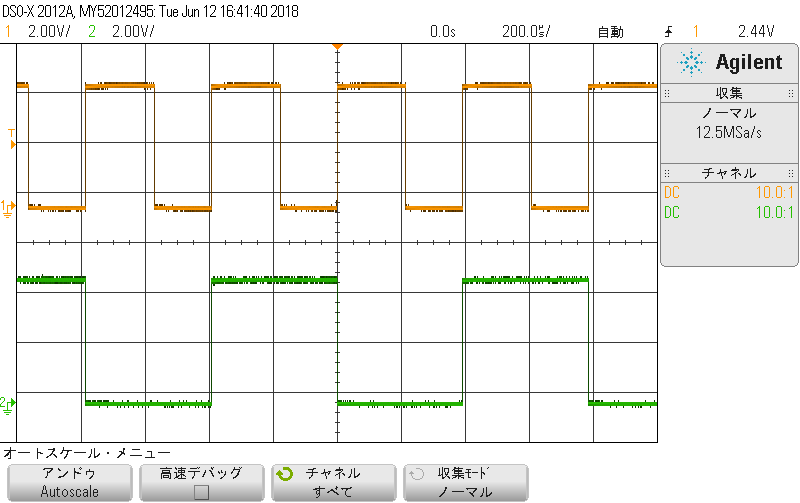
\includegraphics[width=100mm]{scope_06.png}
\label{sample1}\\
\caption{4進カウンタ データ出力$Q_0$の出力波形}
\end{figure}
\par
  \begin{figure}[H]
\centering
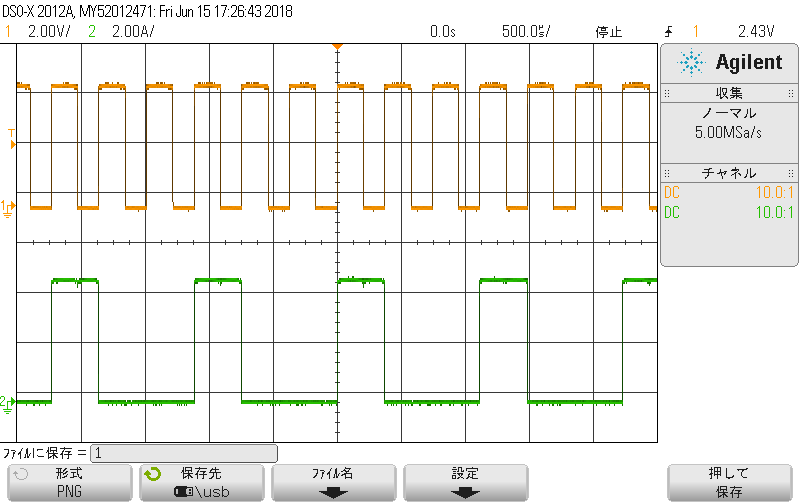
\includegraphics[width=100mm]{1.png}
\label{sample1}\\
\caption{4進カウンタ データ出力$Q_1$の出力波形}
\end{figure}
\par
\begin{figure}[H]
\centering
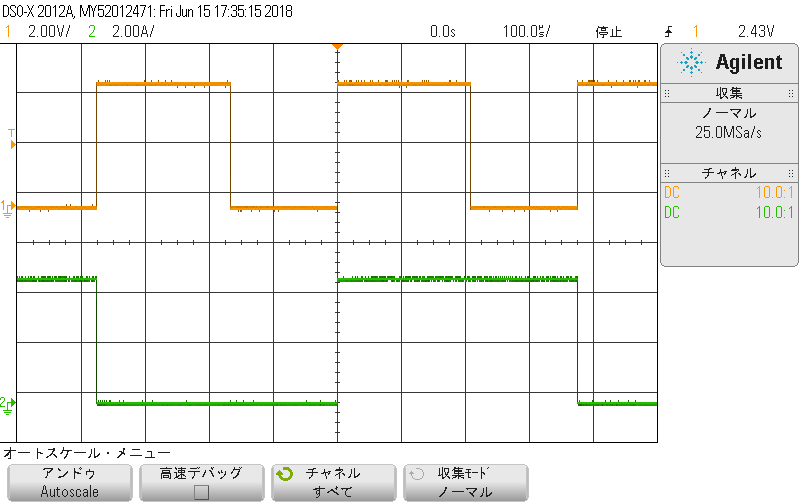
\includegraphics[width=100mm]{2.png}
\label{sample1}\\
\caption{4進カウンタ データ出力$Q_0$と$Q_1$の出力波形}
\end{figure}
\par
 図2からは,出力$Q_0$はクロックが2周期すると1周期する。これから,わかるとようにタイミングチャート
と同じであるため,4新カウンタである。さらに,図3はデータの出力波形$Q_1$が1周期ぶんにクロックが4つ
入っている。そして,図4は出力$Q_0$と$Q_1$の波形を調べ,$Q_1$が1周期経てば,$Q_0$が2周期経つことが
わかる。よって,この図たちから4進カウンタだとわかる。
\item 実験(3) \par
$y_0 = \overline{x}_0 \times \overline{x}_1$\par
$y_1 = x_0$
\begin{figure}[H]
\centering
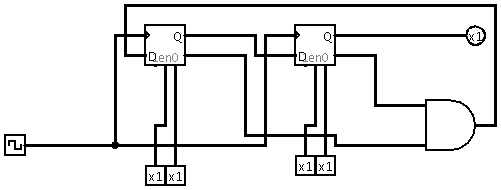
\includegraphics[width=100mm]{sample.png}
\label{sample1}\\
\caption{3進カウンタ 回路図}
\end{figure}
\par
\item 実験(4) \par
\begin{figure}[H]
\centering
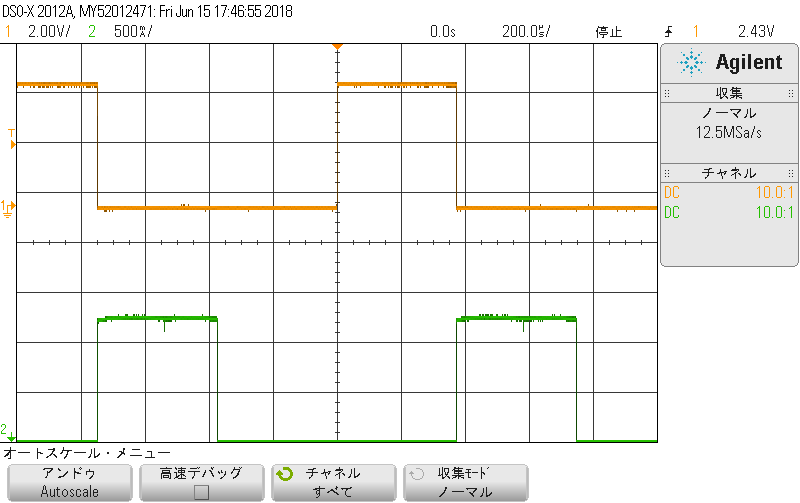
\includegraphics[width=100mm]{3.png}
\label{sample1}\\
\caption{3進カウンタ データ出力Qの出力波形}
\end{figure}
\par
 図6からわかるように,今回はクロックを用いずに出力同士の確認をした。
なぜなら,クロックと出力たちの結果が同じようになっていて違いがわからない。
そのため,出力同士を比べることで差異を見つける。
波形は同じだが,半周期にずれがあり,これにより3進カウンタであるとわかる。
\end{enumerate}

\section{考察}
\begin{enumerate}
  \item 実験自体の考察について
    順序回路は,現在レジスタが保持している値から次の値を求める
  回路が一般的である。しかし,中にはそれだと実現できない回路も存在する。
  それは,次のカウント値を求める際に現在のカウント値の値が異なる回路
  である。小銭のを入力とする自動販売機などが例としてあげられる。例えば,
  今までは1を入力したら次の値が決まっていましたが,小銭だと10円や50円
  ,100円など様々な入力がある。これにより,遷移状態が変わる。よって,初めの
  入力だけでは決まらない。
  \item その他の考察
    今回は,D-FFを使ったレジスタを作成したが,それ以外にもNANDゲートや
  NORゲートを使用したレジスタも回路上では作成可能であるとわかった。
\end{enumerate}

\section{調査課題}
\begin{enumerate}
  \item (a)\par
   シフトレジスタとは,レジスタ内での記憶しているいデータを隣のレジスタに
  移動させる機能を持つレジスタである。データの入力方法では,直列入力型と並列入力型
  ,データのシフト方向では左シフト型,右シフト型に分類できる。\par
    シフトレジスタは,直列に入力されたデータを並列に出力したり,並列に入力されたデータ
  を直列に出力させる変換機能を持つ。さらに,直列入力されたデータを数の分だけクロック入力
  し,最後のレジスタで出力することにより,信号を遅延させる。最後に,シフトができるため
  桁のぶんだけ移動可能だということである。よって,乗算や除算ができる。

\end{enumerate}

\section{感想}
  今回の実験より,カウンタの仕組みを少し理解することができた。記憶回路に
使用したFF(フリップフロップ)は,他のICとは仕組みの違いで戸惑いなどがあり,
あまり進捗状況がよくはなかった。しかし,周りPMや先生たちのおかげで,少しずつ
だが理解しはじめ,作業が進むようになった。
\section{参考文献}
\begin{thebibliography}{9}
 [1]浅川穀 『基礎コンピュータシステム』,東京電機大学出版局, 2004
\end{thebibliography}

\end{document}
